\subsection{The Vertical Line Test}
\begin{definition}[Vertical Line Test]
	This is a test to determine if a graph is a function or not.


\end{definition}

\begin{example}[Non Function] 
	This is not a function because the vertical line passes through 2 points, which means that it outputs more than 1 output.
	\hfill
	\begin{center}
	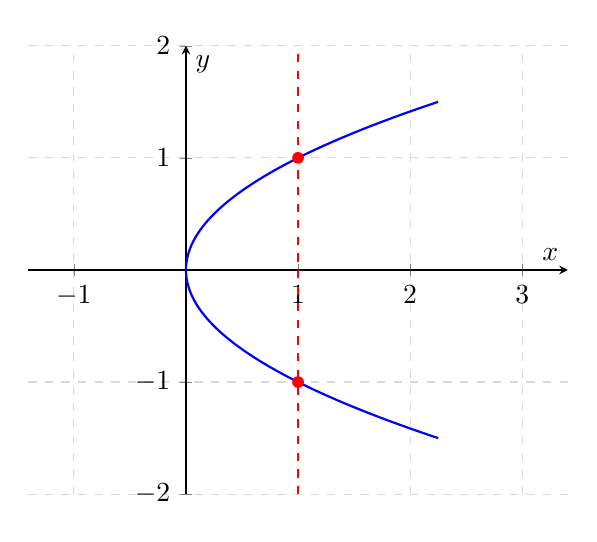
\begin{tikzpicture}
		\begin{axis}[
		    axis lines = center,
		    xlabel = $x$,
		    ylabel = $y$,
		    xmin = -1, xmax = 3,
		    ymin = -2, ymax = 2,
		    grid = both,
		    grid style = {dashed, gray!30},
		    axis equal
		]
		    \addplot [domain=-1.5:1.5, samples=100, thick, blue] ({x^2}, {x});

		    \addplot [red, dashed, thick, no marks] coordinates {(1, -2) (1, 2)};

		    \node[circle, fill=red, inner sep=1.5pt] at (axis cs:1,1) {};
		    \node[circle, fill=red, inner sep=1.5pt] at (axis cs:1,-1) {};
		\end{axis}
	\end{tikzpicture}
	\end{center}
\end{example}

\begin{example}[Function] 
	This is a function because the vertical line passes through only 1 point, which means that it only gives a single output.
	\hfill
	\begin{center}
	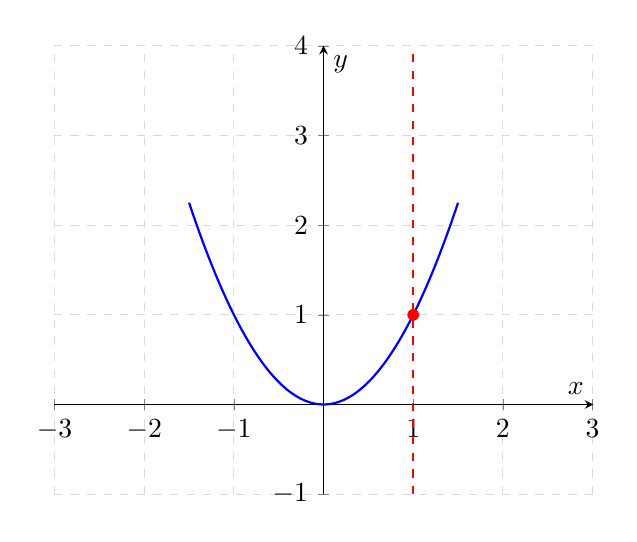
\begin{tikzpicture}
		\begin{axis}[
		    axis lines = center,
		    xlabel = $x$,
		    ylabel = $y$,
		    xmin = -2, xmax = 2,
		    ymin = -1, ymax = 4,
		    grid = both,
		    grid style = {dashed, gray!30},
		    axis equal
		]
		    \addplot [domain=-1.5:1.5, samples=100, thick, blue] {x^2};

		    \addplot [red, dashed, thick, no marks] coordinates {(1, -1) (1, 4)};

		    \node[circle, fill=red, inner sep=1.5pt] at (axis cs:1,1) {};
		\end{axis}
	\end{tikzpicture}
	\end{center}
\end{example}
